%%%%%%%%%%%%%%%%%%%%%%%%%%%%%%%%%%%%%%%%%%%%%%
% Head matter - can we try to be consistent on
% included packages
\documentclass{beamer}
\mode<presentation>
{\usetheme{default}
 \usecolortheme{default}
 \usefonttheme{default}
 \setbeamertemplate{navigation symbols}{}
 \setbeamertemplate{caption}[numbered]} 
\usepackage[english]{babel}
\usepackage[utf8x]{inputenc}
\usepackage{graphicx}
%%%%%%%%%%%%%%%%%%%%%%%%%%%%%%%%%%%%%%%%%%%%%%
% Formatting for title page
\title[First Steps with SCRATCH]{Introduction to Computer Programming\\ Lecture 1: First Steps with SCRATCH}
\author{Sabine Hauert and R.~Eddie Wilson}
\institute{Department of Engineering Mathematics}
\date{30th September 2014}
%%%%%%%%%%%%%%%%%%%%%%%%%%%%%%%%%%%%%%%%%%%%%%
\begin{document}
\begin{frame}
  \titlepage
\end{frame}
%\section{Introduction}
% There is actually no point to the sections 
% since we are not using table of contents mark up
\begin{frame}{Introduction}
\begin{itemize}
  \item Your introduction goes here!
  \item Use \texttt{itemize} to organize your main points.
\end{itemize}
\vskip 1cm
\begin{block}{Examples}
Some examples of commonly used commands and features are included, to help you get started.
\end{block}
\end{frame}

%\section{Some \LaTeX{} Examples}
%\subsection{Tables and Figures}

\begin{frame}{Tables and Figures}
\begin{itemize}
\item Use \texttt{tabular} for basic tables --- see Table~\ref{tab:widgets}, for example.
\item You can upload a figure (JPEG, PNG or PDF) using the files menu. 
\item To include it in your document, use the \texttt{includegraphics} command (see the comment below in the source code).
\end{itemize}

% Commands to include a figure:
%\begin{figure}
%\includegraphics[width=\textwidth]{your-figure's-file-name}
%\caption{\label{fig:your-figure}Caption goes here.}
%\end{figure}

\begin{table}
\centering
\begin{tabular}{l|r}
Item & Quantity \\\hline
Widgets & 42 \\
Gadgets & 13
\end{tabular}
\caption{\label{tab:widgets}An example table.}
\end{table}
\end{frame}


\begin{frame}{Readable Mathematics}
Let $X_1, X_2, \ldots, X_n$ be a sequence of independent and identically distributed random variables with $\text{E}[X_i] = \mu$ and $\text{Var}[X_i] = \sigma^2 < \infty$, and let
$$S_n = \frac{X_1 + X_2 + \cdots + X_n}{n}
      = \frac{1}{n}\sum_{i}^{n} X_i$$
denote their mean. Then as $n$ approaches infinity, the random variables $\sqrt{n}(S_n - \mu)$ converge in distribution to a normal $\mathcal{N}(0, \sigma^2)$.
\end{frame}

\begin{frame}{Eddie shows two columns technique}
\begin{columns}
\begin{column}{0.4\textwidth}
\begin{center}
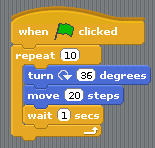
\includegraphics[scale=0.75]{SCRATCHgrab.png}
\end{center}
\end{column}
\begin{column}{0.6\textwidth}
\begin{itemize}
\item This is cleanest way of putting text beside
pictures. 
\item Also illustrating {\tt pause} for reveals --- I 
use this only sparingly
\pause\medskip
\item We need a convention on scaling of included SCRATCH graphics. Here: source image obtained by screen grabbing from desktop SCRATCH 1.4. Hopefully this is consistent across OS etc.! 
\medskip
\item The scaling here is mega-generous - for consideration.
\end{itemize}
% NB \smallskip, \medskip, \bigskip much better for
% consistency than explicit spaces
\end{column}
\end{columns}
\end{frame}


\end{document}